%
%   MIX - I2C - Spec
%

\documentclass[a4paper,12pt]{report}

\setlength{\textwidth}{170mm}
\setlength{\textheight}{255mm}
\setlength{\oddsidemargin}{-5mm}
\setlength{\topmargin}{-18mm}


%\usepackage[OT2,T1]{fontenc}
\usepackage[latin1]{inputenc}
\usepackage{color}
%\usepackage{supertabular}
%\usepackage{epsfig}
\usepackage{graphicx}



\definecolor{brown}{rgb}{0.55,0.32,0.23}
\definecolor{pink}{rgb}{0.79,0.43,0.79}
\definecolor{orange}{rgb}{1,0.76,0.24}

%\usepackage{aaai}


\begin{document}


\begin{titlepage}
\vspace*{70mm}
\centering
\begin{tabular}{p{20mm}l}
\multicolumn{2}{r}{\tt {MIX} - Micronas Interconnect Specification Expander}\\[1mm]
\hline \\[3mm]
&{\bf I2C Sheet - Specification}\\[5mm]
&{\tt Micronas - Munich}\\[5mm]
\hline \\[20mm]
\end{tabular}
\end{titlepage}


\raggedright

\section{General}
The I2C sheet is one more category of input specification. It's content describes I2C Register-blocks and Register connections to Signals of the design core. Signal-names can be used directly because MIX internal uses global signals. By default a new defined Register-block is bound to {\tt TOPLEVEL} (default Language: {\tt VHDL}), this could be changed by adding the Register-blocks Instance manual into the {\tt HIER}-Sheet. If no Instance is defined in {\tt HIER}-Sheet, {\tt MIX} adds this definition interal (Name: {\tt iic\_if\_$<$interface$>$}).

\section{I2C-Sheet details}
The following table describes MIX I2C's header-keywords:

\begin{table}[htb]\begin{tabular}{|l|p{4cm}|p{4cm}|p{15mm}|p{25mm}|}\hline
\begin{bf}Column name\end{bf} & \begin{bf}Descriptionend\end{bf} & \begin{bf}Default value\end{bf} & \begin{bf}Req.\end{bf} & \begin{bf}Example\end{bf}\\\hline
::ign & Ignore line & $<$empty$>$ & man. & \# comm. \\\hline
::variants & Variant selector & Default & opt. & Var1 \\\hline
::width& Register width & 16 & man. & 16 \\\hline
::dev & Device name & n/a & man. & FRCA0 \\\hline
::sub & Sub address & VHDL & opt. & 27 \\\hline
::interface & Domain name & W\_NO\_CONFIG & man. & cc0 \\\hline
::block & Block Name & $<$empty$>$ & opt. & mc \\\hline
::dir & Direction & $<$empty$>$ & opt. & RW \\\hline
::spec & Update Signal & NTO & opt. & takeover\_b72 \\\hline
::clock & Clock Domain & $<$empty$>$ & opt. & clkcc81 \\\hline
::reset & Reset Signal & $<$empty$>$ & opt. & asresc\_n \\\hline
::busy & Busy Signal & $<$empty$>$ & opt. & b81 \\\hline
::b & Bit n & $<$empty$>$ & man. & FMSYN.2 \\\hline
::init & Reset Value & $<$empty$>$ & opt. & 0 \\\hline
::rec & Recommended Value & $<$empty$>$ & opt. & 0 \\\hline
::comment & Comment field & $<$empty$>$ & opt. & This is a comment \\\hline
\end{tabular}\end{table}

\section{I2C-Column details}
\begin{tabular}{lp{14cm}}
  \begin{bf}::ign\end{bf} & Every columns row, conainting \# or // is ignored by MIX\\
  \begin{bf}::variants\end{bf} & Select a line depending on the -variant command line switch. If -variant VAR is set, only lines whose \begin{tt}::variant\end{tt} cell conains the keyword VAR, Default or empty, are selected and  read in. Several variants may be given in one cell, seperated by ",". Without specifying the -variant switch, the "Default" and empty \begin{tt}::variant\end{tt} cells are read in and evaluated.\\
  \begin{bf}::width\end{bf} & Define Register width.\\
  \begin{bf}::dev\end{bf} & Specify the Device address\\
  \begin{bf}::sub\end{bf} & Define Registerblock-subaddress\\
  \begin{bf}::interface\end{bf} & Domain name\\
  \begin{bf}::block\end{bf} & Registerblock Name. The Reistersblock name and its subaddress are building the Instace-name.\\
  \begin{bf}::dir\end{bf} & Defines a Registers input/output direction, possible values are: \begin{tt}R\end{tt}, \begin{tt}W\end{tt} or \begin{tt}RW\end{tt}\\
  \begin{bf}::spec\end{bf} & Update signal\\
  \begin{bf}::clock\end{bf} & set a clock Domain. Every I2C Register may receive it's own clock.\\
  \begin{bf}::reset\end{bf} & Specify a Reset signal. This Signal Resets the I2C Registers.\\
  \begin{bf}::busy\end{bf} & busy signal\\
  \begin{bf}::b\end{bf} & Specifies a signal which is connected to a Regisers pin. This is a multiple column which can be used to set different signals to the same Register\\
  \begin{bf}::init\end{bf} & Set initializing value of register connection(s).\\
  \begin{bf}::rec\end{bf} & Set recommended value of a register connection(s).\\
  \begin{bf}::comment\end{bf} & All entries in these cells are treaten as comments. MIX will keep comments to put them later into VHDL/Verilog output.\\
\end{tabular}
\section{I2C-Sheet input and VHDL output examples}
The following screenshots are showing a small part of  FRCA's I2C sheet. This section describes the \begin{tt}cc0\end{tt} Registerblock which consists of 8 Sub-blocks. Each Sub-blocks Register-connections can be split into multiple rows. This allows you to specify different settings for pins of the same Registerblock.\newline
\newline
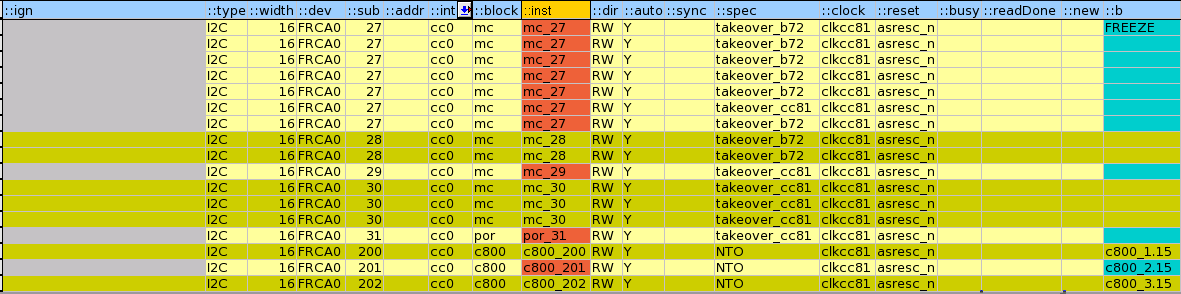
\includegraphics[scale=0.5]{images/FRCA_iic_part0.jpg}\newline
\newline
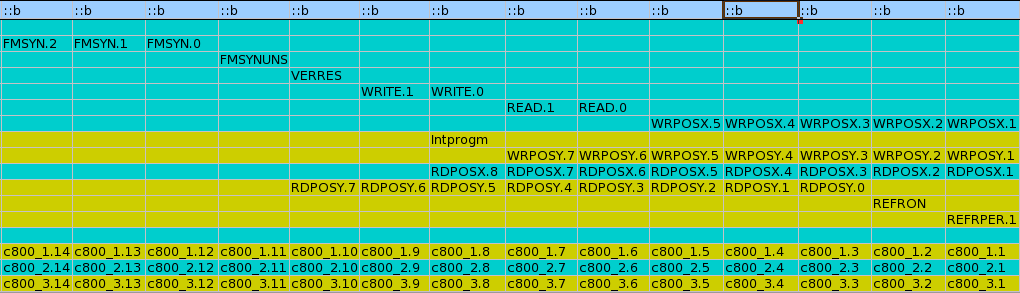
\includegraphics[scale=0.5]{images/FRCA_iic_part1.jpg}\newline
\newline
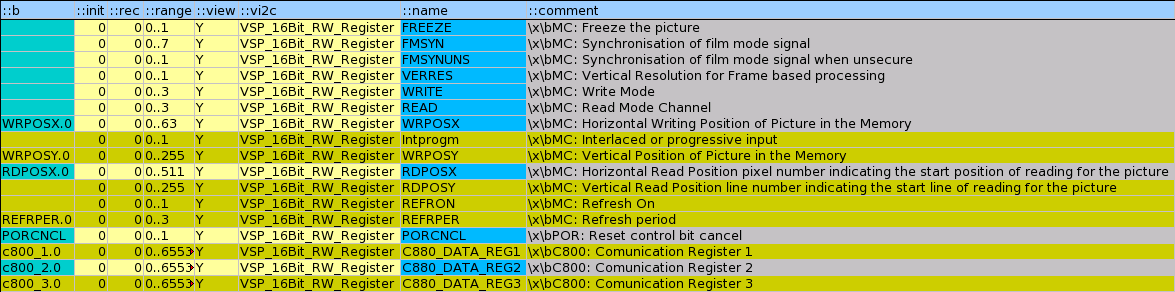
\includegraphics[scale=0.5]{images/FRCA_iic_part2.jpg}\newline
\newline
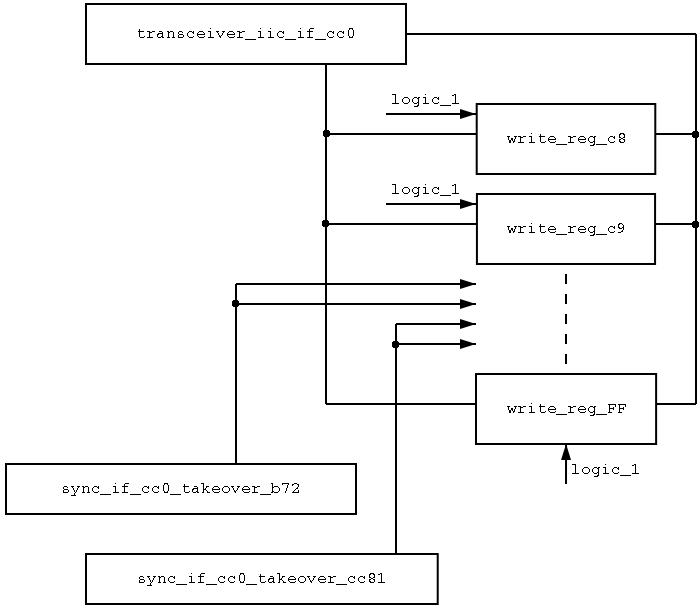
\includegraphics[scale=0.6]{images/FRCA_iic_block.jpg}\newline
\newpage
VHDL Architechture:\newline
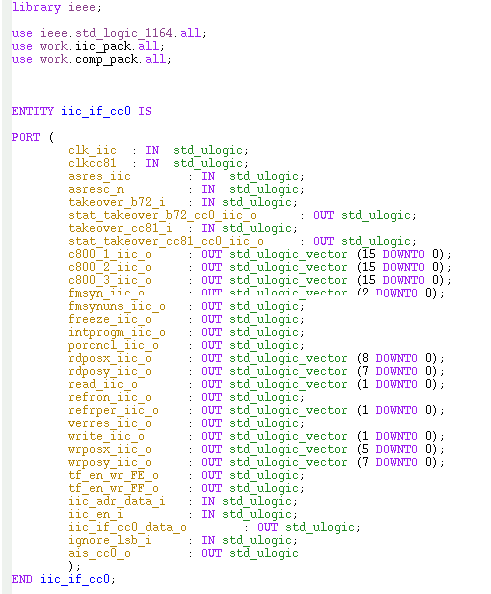
\includegraphics[scale=0.9]{images/FRCA_part_entity.jpg}\newline
\newpage
VHDL Entity (uncomplete):\newline
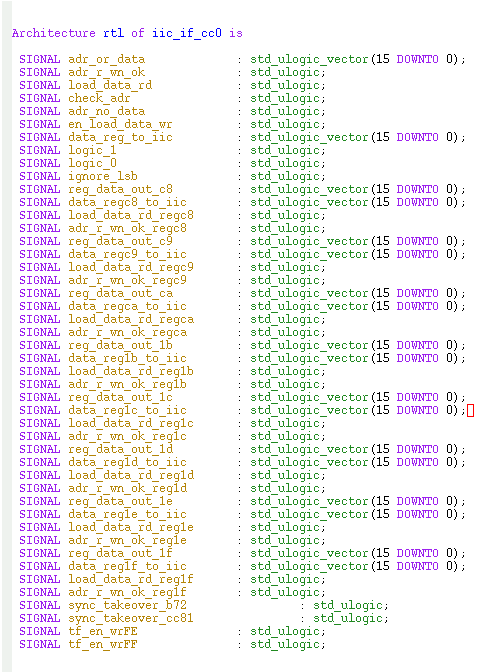
\includegraphics[scale=0.9]{images/FRCA_part0_arch.jpg}\newline
\newline
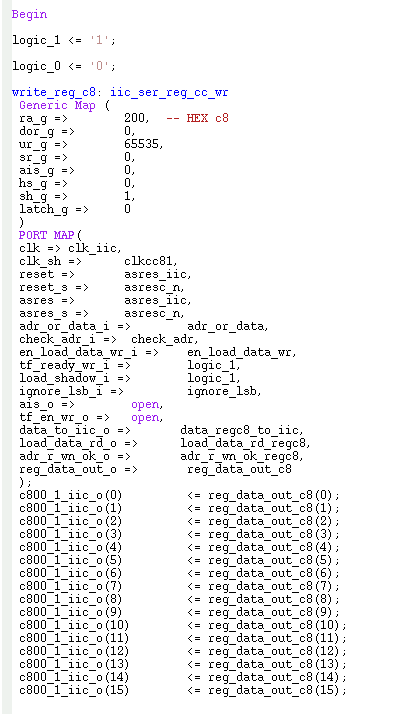
\includegraphics[scale=0.9]{images/FRCA_part1_arch.jpg}\newline
This part of the "\begin{tt}cc0\end{tt}" Architechture only shows the Sub-Address 200 (Hex: \begin{tt}c8\end{tt}). As you can see the Interface-name (or Domainname) will become the Architechture-name while the Subaddress is used to identify the Sub-Registerblock. The Portmap describes connections as told in the I2C Sheet. In the Generic Map you can some I2C specific definitions as "\begin{tt}ra\_g\end{tt}" which hold the Registers Address as "\begin{tt}ur\_g\end{tt}" defines the Port-Range.


\end{document}